\documentclass[aspectratio=169]{beamer}

\usepackage{ccicons}
\usepackage{fontspec}
\usepackage{listings}
\usepackage{tikz}
\usepackage{svg}

\definecolor{uclablue}{RGB}{39,116,174}
\definecolor{uclagold}{RGB}{255,179,0}

\definecolor{ubcorange}{RGB}{158, 66, 37}

\definecolor{cugold}{RGB}{207, 184, 124}
\definecolor{cudarkgray}{RGB}{86, 90, 92}

\definecolor{solarizedred}{RGB}{220, 50, 47}
\definecolor{solarizedblue}{RGB}{38, 139, 210}
\definecolor{solarizedgreen}{RGB}{133, 153, 0}
\definecolor{solarizedpurple}{RGB}{108, 113, 196}
\definecolor{solarizedmagenta}{RGB}{211, 54, 130}

\definecolor{pantone655}{RGB}{0, 42, 92}
\definecolor{pantone7453}{RGB}{123, 164, 217}
\definecolor{pantone633}{RGB}{0, 139, 176}
\definecolor{pantone7492}{RGB}{218, 229, 205}

\colorlet{primarycolor}{pantone655}
\colorlet{secondarycolor}{pantone7453}


\usetikzlibrary{
  arrows,
  arrows.meta,
  automata,
  backgrounds,
  calc,
  chains,
  decorations.pathreplacing,
  fit,
  intersections,
  matrix,
  overlay-beamer-styles,
  positioning,
  shapes,
  shapes.multipart,
  tikzmark,
}
\usetikzmarklibrary{listings}

\hypersetup{
  colorlinks=true,
  urlcolor=cudarkgray,
}

\setbeamercolor{frametitle}{fg=primarycolor}
\setbeamercolor{structure}{fg=primarycolor}
\setbeamercolor{enumerate item}{fg=black}
\setbeamercolor{itemize item}{fg=black}
\setbeamercolor{itemize subitem}{fg=black}

\setbeamersize{text margin left=26.6mm}
\addtolength{\headsep}{2mm}

\setbeamertemplate{navigation symbols}{}
\setbeamertemplate{headline}{}
\setbeamertemplate{footline}{}
\setbeamertemplate{itemize item}{\color{black}}
\setbeamertemplate{itemize items}[circle]

\setbeamertemplate{footline}{
  \begin{tikzpicture}[remember picture,
                      overlay,
                      shift={(current page.south west)}]
    \node [black!50, inner sep=2mm, anchor=south east]
          at (current page.south east) {\footnotesize \insertframenumber};
  \end{tikzpicture}
}

\setsansfont{Inter}[Scale=MatchLowercase]
\setmonofont{Hack}[Scale=MatchLowercase]

\makeatletter
\newcommand\version[1]{\renewcommand\@version{#1}}
\newcommand\@version{}
\def\insertversion{\@version}

\newcommand\lecturenumber[1]{\renewcommand\@lecturenumber{#1}}
\newcommand\@lecturenumber{}
\def\insertlecturenumber{\@lecturenumber}
\makeatother

\setbeamertemplate{title page}
{
  \begin{tikzpicture}[remember picture,
                      overlay,
                      shift={(current page.south west)},
                      background rectangle/.style={fill=pantone655},
                      show background rectangle]
    \node [anchor=west, align=left, inner sep=0, text=white]
          (lecturenumber) at (\paperwidth / 6, \paperheight * 3 / 4)
          {\Large Lecture \insertlecturenumber};
    \node [inner sep=0, align=left, text=white, node distance=0,
          above left=of lecturenumber, anchor=south west, yshift=2mm]
          {\Large ECE 344: Operating Systems};
    \node (title) [inner sep=0, anchor=west, align=left, text=white,
                   text width=30em]
          at (\paperwidth / 6, \paperheight / 2)
          {{\bfseries \Huge \inserttitle{}}};
    \node [inner sep=0, align=right, text=white, node distance=0,
          below right=of title, anchor=north east, yshift=-1mm]
          {{\footnotesize \ttfamily \insertversion}};
    \node [inner sep=0, text=white, align=left, anchor=west]
          (author) at (\paperwidth / 6, \paperheight / 4)
          {\insertauthor};
    \node [text=white, inner sep=0, align=left, node distance=0,
           below left=of author, anchor=north west, yshift=-2mm]
          {\insertdate};
    \node [align=right, anchor=south east, inner sep=2mm, text=white]
          (license) at (\paperwidth, 0)
          {\footnotesize This  work is licensed under a
           \href{http://creativecommons.org/licenses/by-sa/4.0/}
                {\color{pantone7453} Creative Commons Attribution-ShareAlike 4.0
                 International License}};
    \node [text=white, inner sep=0, align=right, node distance=0,
           above right=of license, anchor=south east, xshift=-2mm]
          {\Large \ccbysa};
  \end{tikzpicture}
}

\tikzset{
  >=Straight Barb[],
  shorten >=1pt,
  initial text=,
}

\lstset{
  basicstyle=\footnotesize\ttfamily,
  language=C,
  escapechar=@,
  commentstyle=\color{black!50},
}


\lecturenumber{1}
\title{Overview}
\version{1.0.4}
\author{Jon Eyolfson}
\date{September 8, 2022}

\begin{document}

  \begin{frame}[plain, noframenumbering]
    \titlepage
  \end{frame}

  \begin{frame}
    \frametitle{Hello, I'm Jon}

    I prefer just Jon, but use what you're most comfortable with

    \vspace{2em}

    I'm a new teaching stream professor

    \vspace{2em}

    I've always been interested in computers, and understanding how things work
  \end{frame}

  \begin{frame}
    \frametitle{Prof. Ashvin Goel is the Course Coordinator}

    You'll find the overall course website here:

    \url{https://www.eecg.utoronto.ca/~ashvin/courses/ece344/current/}

    \vspace{2em}

    This is also a Piazza for course discussion
  \end{frame}

  \begin{frame}
    \frametitle{Course Website}

    \url{https://eyolfson.com/courses/ece344/}

    \hspace{2em} If you don't want to logon to Quercus

    \vspace{2em}

    Otherwise, you'll find the material there was well
  \end{frame}

  \begin{frame}
    \frametitle{Lectures}

    We're back in person for the first time in a long time

    \vspace{2em}

    Feel free to raise your hand or ask questions at anytime if anything is
    unclear

    \vspace{2em}

    Coming to class is important, for both yourself and me
  \end{frame}

  \begin{frame}
    \frametitle{Lectures Will Be Streamed with VODs}

    \includegraphics[width=7cm]{../../resources/youtube.eps}

    \vspace{1em}

    \url{https://www.youtube.com/channel/UCRUDk5mnr_ofVRrYqbUk-wQ}
  \end{frame}

  \begin{frame}
    \frametitle{Discussion Will Be Interactive on Discord}

    \includesvg[width=7cm]{../../resources/discord.svg}

    \vspace{1em}

    \url{https://discord.gg/p5SUTrNa9P}

    \vspace{1em}

    \includegraphics[scale=2]{discord-link.eps}
  \end{frame}

  \begin{frame}
    \frametitle{Office Hours Mostly by Appointment}

    I'll primarly be on Discord for offline discussions

    \vspace{2em}

    I'll set office hours based on feedback from Discord

    \vspace{2em}

    These aren't streamed or recorded, this is a resource only for students
  \end{frame}

  \begin{frame}
    \frametitle{There are Quizzes Instead of a Midterm}

    \begin{tabular}{rll}
      \multicolumn{2}{l}{\bfseries Labs (30\% total)} \\
       5\% & Lab 1 & Review of C \\
       6\% & Lab 2 & Cooperative Threads \\
       6\% & Lab 3 & Preemptive Threads \\
       4\% & Lab 4 & Concurrent Web Server \\
       5\% & Lab 5 & Caching Web Server \\
       4\% & Lab 6 & File Systems \\
      \multicolumn{2}{l}{\bfseries Written} \\
      30\% & Quizzes & 3 quizzes throughout the semester (10\% each) \\
      40\% & Final & \\
    \end{tabular}

    Quizzes are online, the first one is September 29th
  \end{frame}

  \begin{frame}
    \frametitle{Academic Honesty}

    You can study together, you cannot do labs or quizzes together

    \vspace{2em}

    Cheating hurts everyone involved

    \vspace{2em}

    Any cheating will not be tolerated
  \end{frame}

  \begin{frame}
    \frametitle{These Books Complement Lectures}

    ``\href{https://www.pearson.com/en-us/subject-catalog/p/modern-operating-systems/P200000003311/9780137538638}
           {Modern Operating Systems}'' \\
    by \href{https://www.cs.vu.nl/~ast/}{Andrew Tanenbaum}

    \vspace{2em}

    ``\href{https://pages.cs.wisc.edu/~remzi/OSTEP/}
           {Operating Systems: Three Easy Pieces}'' \\
    by \href{http://www.cs.wisc.edu/~remzi/}{Remzi Arpaci-Dusseau}
    and \href{http://www.cs.wisc.edu/~dusseau/}{Andrea Arpaci-Dusseau}

    \vspace{2em}

    ``\href{https://en.wikipedia.org/wiki/The_C_Programming_Language}
           {The C Programming Language}'' \\
    by \href{https://en.wikipedia.org/wiki/Brian_Kernighan}{Brian Kernighan}
    and \href{https://en.wikipedia.org/wiki/Dennis_Ritchie}{Dennis Ritchie}
  \end{frame}

  \begin{frame}
    \frametitle{Please Provide Feedback}

    I want you to get the most out of this course

    \vspace{2em}

    Let me know what you like, dislike, or want to see more of

    \vspace{2em}

    I'm open to suggestions!
  \end{frame}
  
  \begin{frame}
    \vfill
    ``All problems in computer science can be solved by another level of
    indirection''

    \begin{flushright}
      - David Wheeler
    \end{flushright}
    \vfill
  \end{frame}

  \begin{frame}
    \frametitle{An Operating System Sits between Applications and Hardware}

    \centering
    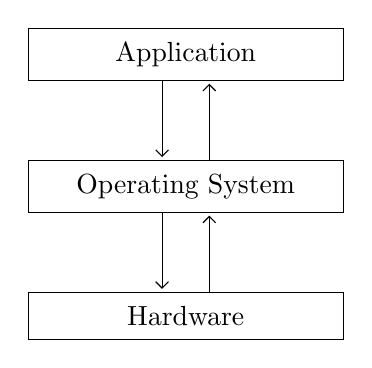
\begin{tikzpicture}[every node/.style={draw, minimum width=4cm, inner sep=0.5em}]
      \node (app) {Application};
      \node [below=of app] (os) {Operating System};
      \node [below=of os] (hw) {Hardware};

      \draw [->, transform canvas={xshift=-3mm}] (app) -- (os);
      \draw [->, transform canvas={xshift=3mm}] (os) -- (app);

      \draw [->, transform canvas={xshift=-3mm}] (os) -- (hw);
      \draw [->, transform canvas={xshift=3mm}] (hw) -- (os);
    \end{tikzpicture}

    \begin{flushright}
      The primary role of an operating system is to manage and coordinate resources
    \end{flushright}
  \end{frame}

  \begin{frame}
    \frametitle{Ubuntu and Android are Considered Different Operating Systems}

    Both use a Linux kernel, but they run different applications

    \vspace{2em}

    There isn't a clear line, especially with ``Linux''

    \vspace{4em}

    For desktop applications, you'd draw the line at the Display System

    \vspace{2em}

    ``Linux'' uses Wayland, and Android uses SurfaceFlinger
  \end{frame}

  \begin{frame}
    \frametitle{Operating Systems Allow Running More than One Application}

    Without an operating system, a CPU starts executing code at a fixed address

    \vspace{4em}

    You could put your application here, but it would be the only one

    \vspace{2em}

    You would have to handle specific hardware in your application

    \vspace{4em}

    Instead, we start executing an operating system at boot
  \end{frame}

  \begin{frame}
    \frametitle{Our First Abstraction is a Process}

    Each process contains its own set of registers, including the program counter

    \vspace{2em}
    
    When starting a process, it specifies where the CPU should start executing

    \vspace{4em}

    The operating systems has to:
    \begin{itemize}
      \item Keeps track of registers for each process
      \item Switch between different processes
      \item Decide when to switch between processes
    \end{itemize}
  \end{frame}

  \begin{frame}
    \frametitle{We Could Put Applications in Different Parts of Memory}

    \centering
    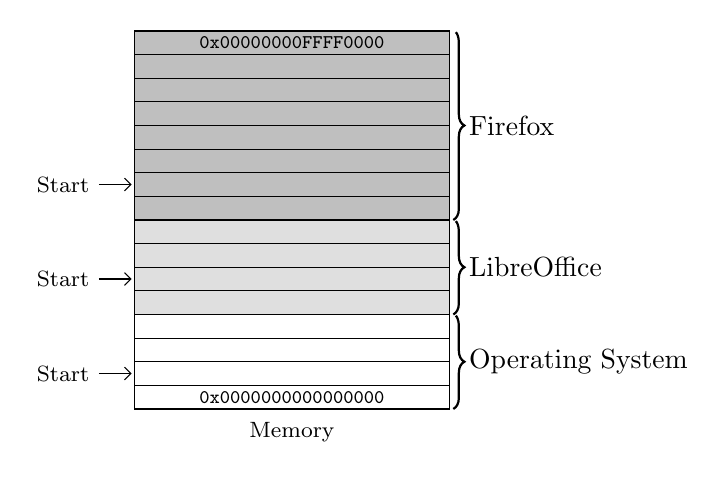
\begin{tikzpicture}
      \node [align=center] at (2, 0) {\footnotesize Memory};
      \draw [fill=black!25] (0, 2.7) rectangle (4, 5.1);
      \draw [fill=black!12.5] (0, 1.5) rectangle (4, 2.7);
      \node [align=center] at (2, 0.45) {\scriptsize \ttfamily 0x0000000000000000};
      \node [align=center] at (2, 4.95) {\scriptsize \ttfamily 0x00000000FFFF0000};
      \foreach \i in {1, ..., 16}
      {
        \draw (0, 0.3 * \i) rectangle (4, \i * 0.3 + 0.3);
      }
      \draw [decorate, decoration={brace, amplitude=4pt, mirror}, thick]
        (4.05, 0.3) -- (4.05, 1.5) node [midway, anchor=west, xshift=0.2em]
        {Operating System};
      \draw [decorate, decoration={brace, amplitude=4pt, mirror}, thick]
        (4.05, 1.5) -- (4.05, 2.7) node [midway, anchor=west, xshift=0.2em]
        {LibreOffice};
      \draw [decorate, decoration={brace, amplitude=4pt, mirror}, thick]
        (4.05, 2.7) -- (4.05, 5.1) node [midway, anchor=west, xshift=0.2em]
        {Firefox};

      \draw [->] (-0.45, 0.75) -- (0, 0.75) node [pos=0, anchor=east] {\footnotesize Start};
      \draw [->] (-0.45, 1.95) -- (0, 1.95) node [pos=0, anchor=east] {\footnotesize Start};
      \draw [->] (-0.45, 3.15) -- (0, 3.15) node [pos=0, anchor=east] {\footnotesize Start};
    \end{tikzpicture}

    \begin{flushright}
      This isn't very flexible
    \end{flushright}
  \end{frame}

  \begin{frame}
    \frametitle{Virtualization Fools Something into Thinking it Has All Resources}

    \begin{columns}[c]
      \column{0.5\textwidth}
      \flushright
    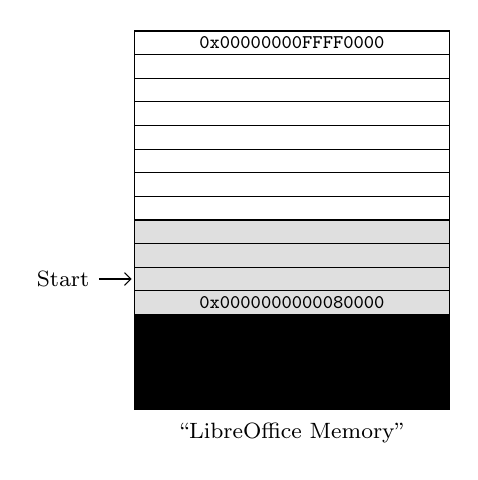
\begin{tikzpicture}
      \node [align=center] at (2, 0) {\footnotesize ``LibreOffice Memory''};
      \draw [fill=black] (0, 0.3) rectangle (4, 1.5);
      \draw [fill=black!12.5] (0, 1.5) rectangle (4, 2.7);
      \node [align=center] at (2, 1.65) {\scriptsize \ttfamily 0x0000000000080000};
      \node [align=center] at (2, 4.95) {\scriptsize \ttfamily 0x00000000FFFF0000};
      \foreach \i in {1, ..., 16}
      {
        \draw (0, 0.3 * \i) rectangle (4, \i * 0.3 + 0.3);
      }

      \draw [->] (-0.45, 1.95) -- (0, 1.95) node [pos=0, anchor=east] {\footnotesize Start};
    \end{tikzpicture}
      \column{0.5\textwidth}
      \flushleft
    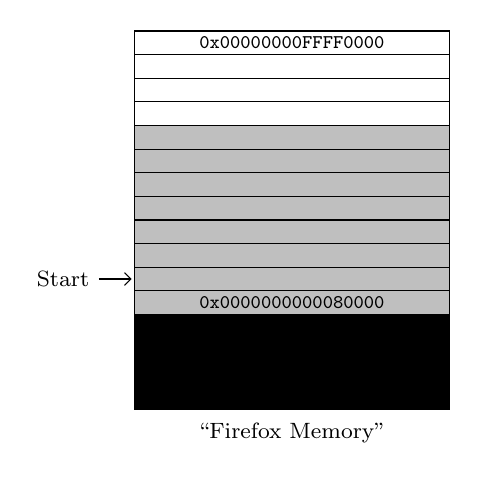
\begin{tikzpicture}
      \node [align=center] at (2, 0) {\footnotesize ``Firefox Memory''};
      \draw [fill=black] (0, 0.3) rectangle (4, 1.5);
      \draw [fill=black!25] (0, 1.5) rectangle (4, 3.9);
      \node [align=center] at (2, 1.65) {\scriptsize \ttfamily 0x0000000000080000};
      \node [align=center] at (2, 4.95) {\scriptsize \ttfamily 0x00000000FFFF0000};
      \foreach \i in {1, ..., 16}
      {
        \draw (0, 0.3 * \i) rectangle (4, \i * 0.3 + 0.3);
      }

      \draw [->] (-0.45, 1.95) -- (0, 1.95) node [pos=0, anchor=east] {\footnotesize Start};
    \end{tikzpicture}
    \end{columns}
  \end{frame}

  \begin{frame}
    \frametitle{Virtual Memory Abstracts Away Physical Memory}

    Each process believes it has access to all the memory

    \vspace{2em}

    Different processes can have the same starting address


    \vspace{4em}

    The operating system has to:
    \begin{itemize}
      \item Map virtual memory access to physical memory
      \item Keep track of memory usage (allocate and deallocate)
      \item Handle out-of-memory scenarios
    \end{itemize}
  \end{frame}

  \begin{frame}
    \frametitle{Virtualization is a Powerful Concept}

    Applies to both processes and virtual memory

    \vspace{4em}

    We can extend this to an entire machine

    \vspace{2em}

    A single physical machine can run multiple operating systems at once
  \end{frame}

  \begin{frame}
    \frametitle{Concurrency is Multiple Things Happening at the Same Time}

    We want multiple applications running at once

    \vspace{2em}

    We want applications to do multiple things at once

    \vspace{4em}

    We don't want applications isolated

    \vspace{2em}

    We want applications and libraries to communicate   
  \end{frame}

  \begin{frame}
    \frametitle{Concurrency is Necessary for Operating Systems}

    Running one application at a time isn't a good experience

    \vspace{2em}

    Completely isolated applications aren't useful

    \hspace{2em} The simplest applications still communicate with the terminal

    \vspace{4em}

    The operating system has to:
    \begin{itemize}
      \item Allow multiple executions at once, safely
      \item Manage abstractions for different kinds of inter-process communication (IPC)
      \item Provide permission checking and access control
    \end{itemize}
  \end{frame}

  \begin{frame}
    \frametitle{Finally, We Need Persistence for a Basic Operating System}

    We want to be able to access data between boots

    \vspace{2em}

    A file system specifies how to organize data on a storage medium

    \vspace{4em}
    
    The operating system has to:
    \begin{itemize}
      \item Store and retrieve data
      \item Ensure integrity of data
    \end{itemize}
  \end{frame}

  \begin{frame}
    \frametitle{File Descriptors Abstract Both Communication and Persistence}

    A file descriptor is just a number identifier (per process) that you can:
    \begin{itemize}
      \item Read bytes from
      \item Write bytes to 
    \end{itemize}

    \vspace{4em}

    The operating system can direct the bytes to whatever it represents

    \vspace{2em}

    You could imagine it representing a file, or one side of communication
  \end{frame}

  \begin{frame}
    \frametitle{Most Kernel Code is Device Drivers}

    Device drivers implement the abstractions we'll learn to the physical hardware

    \vspace{2em}

    It involves reading manufacturer specifications, and finding bugs

    \vspace{2em}

    Sometimes there's inconsistencies between documentation and reality
  \end{frame}

  \begin{frame}[fragile]
    \frametitle{An Actual Comment Linux Source (\texttt{arch/x86/kernel/apm\_32.c})}
    \begin{lstlisting}
/*
 *  Check for clue free BIOS implementations who use
 *  the following QA technique
 *
 *      [ Write BIOS Code ]<------
 *               |                ^
 *      < Does it Compile >----N--
 *               |Y               ^
 *      < Does it Boot Win98 >-N--
 *               |Y
 *           [Ship It]
 *
 *      Phoenix A04  08/24/2000 is known bad (Dell Inspiron 5000e)
 *      Phoenix A07  09/29/2000 is known good (Dell Inspiron 5000)
 */
    \end{lstlisting}
  \end{frame}

  \begin{frame}
    \frametitle{Believe It or Not, This Is ``Hello World''}

    \scriptsize \ttfamily
    0x7F 0x45 0x4C 0x46 0x02 0x01 0x01 0x00 0x00 0x00 0x00 0x00 0x00 0x00 0x00
    0x00
    
    0x02 0x00 0xB7 0x00 0x01 0x00 0x00 0x00 0x78 0x00 0x01 0x00 0x00 0x00 0x00
    0x00
    
    0x40 0x00 0x00 0x00 0x00 0x00 0x00 0x00 0x00 0x00 0x00 0x00 0x00 0x00 0x00
    0x00
    
    0x00 0x00 0x00 0x00 0x40 0x00 0x38 0x00 0x01 0x00 0x40 0x00 0x00 0x00 0x00
    0x00
    
    0x01 0x00 0x00 0x00 0x05 0x00 0x00 0x00 0x00 0x00 0x00 0x00 0x00 0x00 0x00
    0x00
    
    0x00 0x00 0x01 0x00 0x00 0x00 0x00 0x00 0x00 0x00 0x01 0x00 0x00 0x00 0x00
    0x00
    
    0xA8 0x00 0x00 0x00 0x00 0x00 0x00 0x00 0xA8 0x00 0x00 0x00 0x00 0x00 0x00
    0x00
    
    0x00 0x10 0x00 0x00 0x00 0x00 0x00 0x00 0x08 0x08 0x80 0xD2 0x20 0x00 0x80
    0xD2
    
    0x81 0x13 0x80 0xD2 0x21 0x00 0xA0 0xF2 0x82 0x01 0x80 0xD2 0x01 0x00 0x00
    0xD4
    
    0xC8 0x0B 0x80 0xD2 0x00 0x00 0x80 0xD2 0x01 0x00 0x00 0xD4 0x48 0x65 0x6C
    0x6C
    
    0x6F 0x20 0x77 0x6F 0x72 0x6C 0x64 0x0A
  \end{frame}

  \begin{frame}
    \frametitle{There are 3 Major Concepts in This Course}

    You'll learn how the following applies to operating systems:
    \begin{itemize}
      \item Virtualization
      \item Concurrency
      \item Persistence
    \end{itemize}
  \end{frame}
\end{document}
